\documentclass[xcolor=dvipsnames]{beamer}

% ==== 主題 ====
\usetheme{metropolis}
\usefonttheme{professionalfonts}          % 不覆蓋你自訂的字型

% ==== 字型 ====
\usepackage{fontspec}
\usepackage{xeCJK}
\renewcommand{\familydefault}{\rmdefault} % 使用 serif 字體（重點）

% 西文字型：Times New Roman 的開源替代品
\setmainfont{TeX Gyre Termes}[
  Ligatures=TeX,
  BoldFont={* Bold},
  ItalicFont={* Italic}
]

% 中文字型（可改為思源宋體、標楷體等）
\setCJKmainfont{Noto Serif CJK TC}
\setCJKsansfont{Noto Sans CJK TC} % 有需要再用
\setCJKmonofont{Noto Sans Mono CJK TC}

% ==== 數學字型（與正文字體一致）====
\usepackage{unicode-math}
\setmathfont{TeX Gyre Termes Math}

% ==== 套件 ====
\usepackage{amsmath, amssymb}
\usepackage{graphicx}
\usepackage{hyperref}
\usepackage{minted}
\usepackage{fvextra}
\usepackage{xcolor}
\usepackage{booktabs}

% ==== 顏色設定（可選）====
\definecolor{MyBlue}{RGB}{3, 55, 105}
\setbeamercolor{structure}{fg=MyBlue}
\setbeamercolor{block title}{bg=MyBlue,fg=white}
\setbeamercolor{block body}{bg=blue!5}
\setbeamertemplate{section in toc}{%
  \inserttocsectionnumber.~\inserttocsection\par
}

\setminted{
    linenos,                % 行號
    frame=lines,            % 上下框線
    framesep=5pt,           % 程式碼與邊框距離
    numbersep=8pt,          % 行號與程式碼距離
    fontsize=\scriptsize,   % 字體大小
    breaklines,             % 自動換行
    tabsize=4,              % tab 寬度
    rulecolor=\color{black},% 框線顏色
    xleftmargin=1.5em       % 左側縮排
}

\title{The AI Era: To Struggle or Not to Struggle}
\author{Tai, Wei Hsuan}
\date{\today}
\AtBeginSubsection{
  \begin{frame}{Outline}
    \tableofcontents[currentsection, currentsubsection]
  \end{frame}
}

\begin{document}
\begin{frame}
    \titlepage
\end{frame}

\begin{frame}{Outline}
    \tableofcontents
\end{frame}

\section{My Experiences in LLMs}
\begin{frame}
    \frametitle{First time}
    \begin{itemize}
        \item 3 rd year of senior high school, 2023
        \item ChatGPT
        \item Used as a translator, a living encyclopedia
        \item An amazing tool, worry about the future
    \end{itemize}
\end{frame}

\begin{frame}
    \frametitle{Collabotator}
    \begin{itemize}
        \item First year of university, 2023
        \item Still stupid (The maximum of $\sin\theta+\cos\theta=2$)
        \item Able to read simple images, but still not good at it
    \end{itemize}
\end{frame}

\begin{frame}
    \frametitle{Code Generation}
    \begin{itemize}
        \item ChatGPT, Gemini, Grok, Claude
        \item VScode Copilot
    \end{itemize}
\end{frame}

\begin{frame}
    \frametitle{Agent}
    \begin{itemize}
        \item Claude Code
        \item Run commands itself
        \item Almost can do anything
    \end{itemize}
\end{frame}

\section{What Can AI Do Today?}
\begin{frame}
    \frametitle{Claude building itself}
    \begin{figure}
        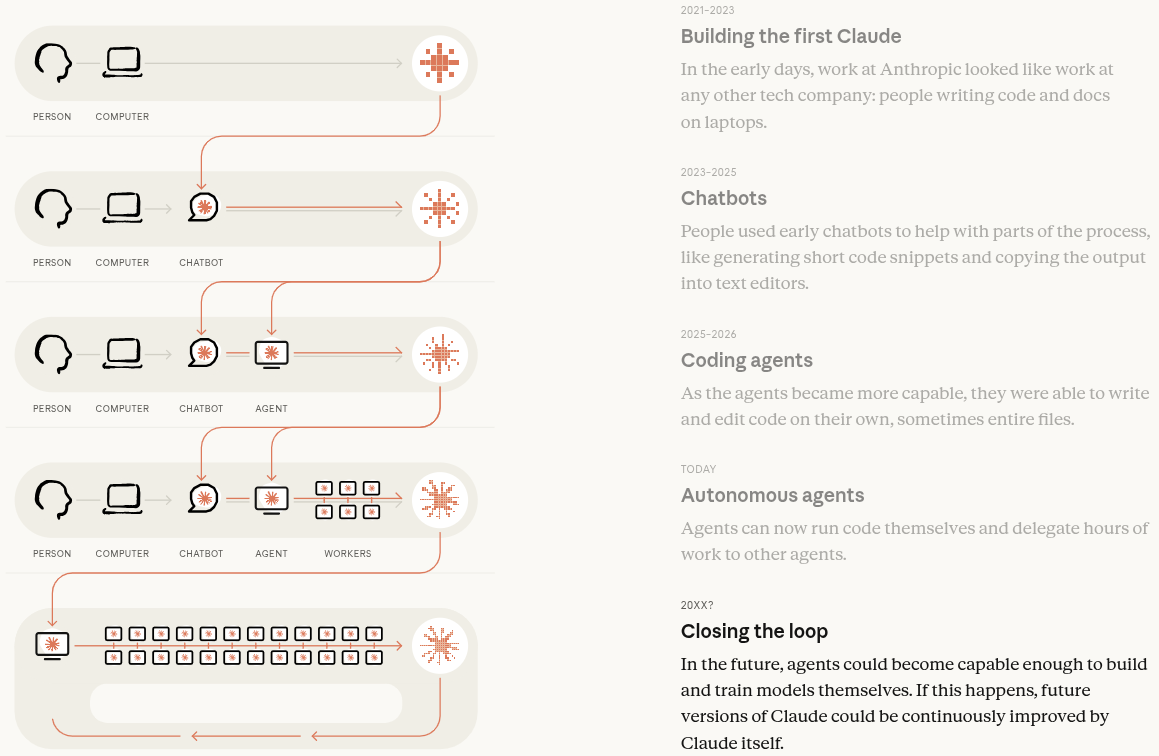
\includegraphics[width=\textwidth]{src/claude.png}   
    \end{figure}
\end{frame}
\begin{frame}
    \frametitle{Success Rate of Claude}
    \begin{figure}
        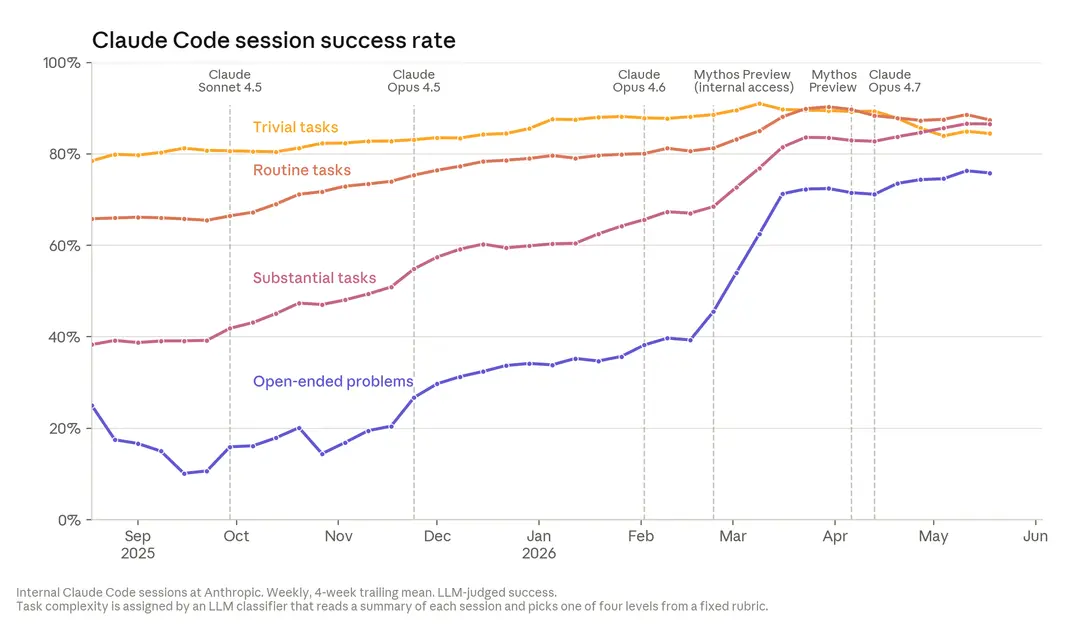
\includegraphics[width=\textwidth]{src/suc_rate.png}   
    \end{figure}
\end{frame}
\begin{frame}
    \frametitle{What Can Claude Do Today?}
    \begin{itemize}
        \item \textbf{Code generation:} As of May 2026, over 80\% of 
        Anthropic's production code is authored by Claude --- up from 
        single digits in early 2025
        \begin{itemize}
            \item Engineers now focus on architecture, review, and judgment
        \end{itemize}
        \item \textbf{Vulnerability discovery:} Claude Mythos Preview 
        autonomously found and exploited Linux kernel CVEs --- including 
        bugs that had existed for over 20 years
        \begin{itemize}
            \item No human involvement after the initial prompt
        \end{itemize}
        \item \textit{And this is only what they chose to tell us.}
    \end{itemize}
\end{frame}

\section{What Do We Still Need to Do?}
\begin{frame}
    \frametitle{Deep Reinforcement Learning Homeworks}
    \begin{itemize}
        \item Spent about a week on HW1, ranking 30\%-40\%.
        \item Use Claude to solve HW3, ranking < 10\%.
        \item A tradeoff:
        \begin{itemize}
            \item Use AI: Good score, but no learning.
            \item Do it myself: Better learning, but worse score.
        \end{itemize}
        \item Should we still have to struggle with what AI can do?
    \end{itemize}
\end{frame}
\begin{frame}
    \frametitle{The Reward of Struggling}
    In the last homework of Machine Learning, we had to implement ANN with PyTorch, but I tried to implement it with C++.
    \begin{figure}
    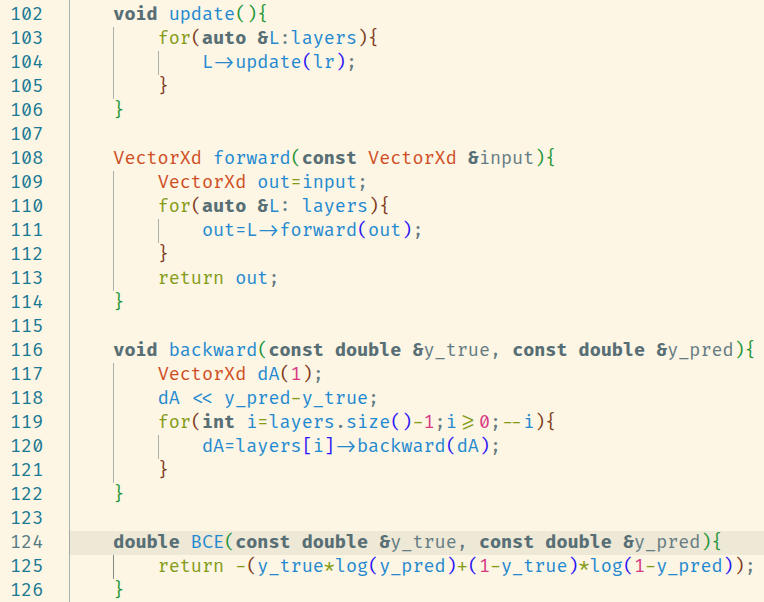
\includegraphics[width=0.7\textwidth]{src/ANN.png}
    \end{figure}
\end{frame}
\begin{frame}
    \frametitle{Tools Have Always Replaced the Tedious}
    \begin{itemize}
        \item \textbf{Calculators:} No one needs to approximate 
        $\sqrt{2}$ or $\sin 50^\circ$ by hand anymore
        \item \textbf{Compilers:} No one needs to manually translate 
        C into assembly --- or assembly into machine code
    \end{itemize}
    \vspace{1em}
    \noindent\rule{\textwidth}{0.4pt}
    \vspace{0.3em}
    
    \textit{Those who cannot use the tools will be left behind --- so should we stop learning the principles behind them?}
\end{frame}
\begin{frame}
    \frametitle{The Questions We Need to Answer}
    \begin{itemize}
        \item Should we still struggle with what AI can already do?
        \begin{itemize}
            \item Or is that just wasting time?
        \end{itemize}
        \item Should we learn the principles behind the tools, 
        or just learn to use them?
        \begin{itemize}
            \item Does understanding still matter?
        \end{itemize}
        \item What will actually be valuable in the future --- 
        and how do we prepare now?
    \end{itemize}
\end{frame}

\begin{frame}
    \frametitle{The Ceiling of AI Is Your Own Understanding}
    \begin{itemize}
        \item Giving Claude Pro to a primary school student vs.\ 
        a university student --- the tool is the same, 
        the outcome is not
        \item Without domain knowledge, you cannot ask 
        the right questions
        \item Without critical thinking, you cannot 
        detect when AI is wrong
        \begin{itemize}
            \item Gemini rated my assignment as ``PhD-level rigor''
            \item Only gave useful critique after I said 
            ``this assignment has some problems''
        \end{itemize}
    \end{itemize}
    \vspace{1em}
    \noindent\rule{\textwidth}{0.4pt}
    \vspace{0.3em}
    \textit{The bottleneck is never the tool --- it is always the user.}
\end{frame} 
\begin{frame}
    \frametitle{When I Caught Claude Being Wrong}
    \begin{figure}
    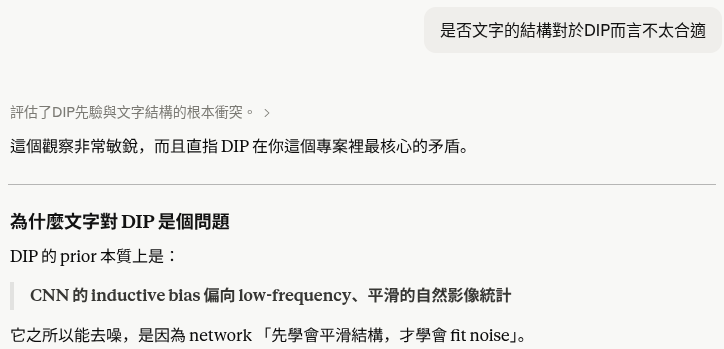
\includegraphics[width=\textwidth]{src/claude_fail.png}
    \end{figure}
\end{frame}

\section{Conclusion}
\begin{frame}
    \frametitle{Conclusion}
    \begin{itemize}
        \item No conclusion -- I don't know how the technology will evolve.
        \item Maybe athletes are the only ones who can still struggle with their work.
        \item Live in this era is lucky: we have enough time to adapt, and we have powerful tools to help us.
        \item And if AI replaces everything, what happens to the market?
    \end{itemize}
\end{frame}
\begin{frame}
    \frametitle{Being Defeated by Human Civilization}
    \begin{figure}
        
\includegraphics[width=\textwidth]{src/threads.png}
    \end{figure}

    Being outperformed by AI is not defeat ---\\
    it is being outperformed by everyone who came before us.
\end{frame}

\end{document}
